\documentclass[MAIN.tex]{subfiles} 
\begin{document} 
	%======================================================================================= %
	\begin{frame}[fragile]
		\frametitle{The Exponential Distribution}

\textbf{The Exponential Distribution}

\item The exponential distribution is often used to model the waiting time X between events occurring randomly and independently in time (or space).\item  Because it is a continuous distribution, the height of the exponential curve at any X refers to probability density rather than probability.
\item  Probability is instead represented by area under the exponential curve.
\end{itemize}

\end{frame}	
%======================================================================================= %

\begin{frame}
\textbf{The Exponential Distribution}
	\begin{figure}
\centering
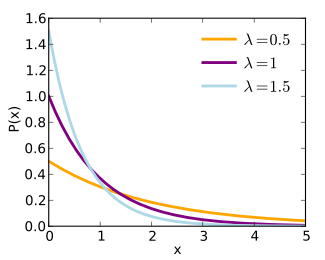
\includegraphics[width=0.7\linewidth]{images/exponential}
\end{figure}
\end{frame}
%===============================================================================%
\begin{frame}[fragile]
	\frametitle{The Exponential Distribution}
		

\item The main assumption of the exponential distribution is that at any point in time, the probability of an event occurring in the next instant does not depend on how much time has already elapsed since the previous event. 
\item The parameter of the exponential distribution is the \textbf{rate parameter} at which events occur (the number of events per unit time). \item The mean of the exponential distribution is 1/rate.
\end{itemize}

\end{frame}
%===============================================================================%
\begin{frame}[fragile]
	\frametitle{The Exponential Distribution}
	

Waiting time X to the next event has probability density

\begin{framed}
\begin{verbatim}
dexp(X, rate=1)
dexp(X, rate=1, log=TRUE)
\end{verbatim}
\end{framed}
The default value for the rate is 1, so you must alter to fit your circumstance.

\end{frame}

%%======================================================================================== %
%\subsection{The Exponential Distribution}
%
%
%The exponential distribution describes the arrival time of a randomly recurring independent event sequence. If $\mu$ is the mean ``duration" or ``waiting time" for the next event recurrence, its probability density function is given as
%
%\[f(x;\lambda) = \begin{cases}
%\lambda e^{-\lambda x}, & x \ge 0, \\
%0, & x < 0.
%\end{cases}\]
%The parameter $\lambda$  is called \textbf{\emph{rate}} parameter. It is the inverse of the expected duration ($\mu$).\\
%\[\mu= \frac{1}{\lambda}\].The cumulative distribution function of an exponential distribution is
%
%\[
%F(x;\lambda) = \begin{cases}
%1-e^{-\lambda x}, & x \ge 0, \\
%0, & x < 0.
%\end{cases}\]
%
%If the expected duration is 5 ( e.g. five minutes) then the rate parameter value is 0.2. When implemented with \texttt{R}, the exponential distribution is characterized by the single parameter \texttt{\textbf{rate}}.The commands follow the same kind of naming convention, and the names of the commands are \texttt{\textbf{dexp()}}, \texttt{\textbf{pexp()}}, \texttt{\textbf{qexp()}}, and \texttt{\textbf{rexp()}}. A few examples are given below to show how to use the various commands. 
%===============================================================================%
\begin{frame}[fragile]
	\frametitle{Exponential Distribution : Problem}
	


\item The mean checkout time of a supermarket cashier is three minutes. 
\item Find the probability of a customer checkout being completed by the cashier in less than two minutes, three minutes and four minutes. 
\item (i.e. what percentage of ``waiting times" are less than two, three and four minutes?)
\end{itemize}
\end{frame}
%===============================================================================%
\begin{frame}[fragile]
	\frametitle{The Exponential Distribution}
	
\textbf{\emph{Solution}} 

\item The checkout processing rate is equals to one divided by the mean checkout completion time. 
\item Hence the processing rate is 1/3 checkouts per minute. 
\item We then apply the function \texttt{\textbf{pexp()}} of the exponential distribution with rate=1/3.
\end{itemize} 

\begin{framed}
\begin{verbatim}
> pexp(2,rate=1/3)
[1] 0.4865829
>
> pexp(3,rate=1/3)
[1] 0.6321206
>
> pexp(4,rate=1/3)
[1] 0.7364029
>
> pexp(5,rate=1/3,lower=FALSE)
[1] 0.1888756
\end{verbatim}
\end{framed}
\end{frame}
%%===============================================================================%
%\begin{frame}[fragile]
%	\frametitle{The Exponential Distribution}
%	
%The probabilities of finishing a checkout in under two, three and four minutes by the cashier are approximately 48.6 \%, 63.21\% and 73.6\% respectively. 


\item What is the median waiting time? To answer this question we would use the \texttt{\textbf{qexp()}} function.
\item Recall that the median is value of $x$ such that $P(X \leq x) = 0.50$.
\item Also determine the first and third quartiles $Q_1$ and $Q_3$.

\begin{verbatim}
> qexp(0.5,rate=1/3)
[1] 2.079442
> qexp(0.25,rate=1/3)
[1] 0.8630462
> qexp(0.75,rate=1/3)
[1] 4.158883
\end{verbatim}
